\documentclass[onecolumn,draftclsnofoot, 10pt, compsoc]{IEEEtran}

\usepackage{graphicx}
\usepackage[section]{placeins}
\usepackage{caption}

\usepackage{amssymb}                                         
\usepackage{amsmath}                                         
\usepackage{amsthm}                                

\usepackage{alltt}                                           
\usepackage{float}
\usepackage{color}
\usepackage{url}

\usepackage{balance}
\usepackage[TABBOTCAP, tight]{subfigure}
\usepackage{enumitem}
\usepackage{pstricks, pst-node}
\usepackage{url}
\usepackage{setspace}

\usepackage{etoolbox}
\AtBeginEnvironment{quote}{\singlespacing\vspace{-\topsep}\small}

%\input{pygments.tex}

\usepackage{geometry}
\geometry{left=0.75in,right=0.75in,top=0.75in,bottom=0.75in}
\parindent = 0.0 in
\parskip = 0.1 in

\usepackage{listings}
\lstset{language=C,caption={Descriptive Caption Text},label=DescriptiveLabel}
\lstdefinestyle{customc}{
	belowcaptionskip=1\baselineskip,
	breaklines=true,
	frame=L,
	xleftmargin=\parindent,
	language=C,
	showstringspaces=false,
	basicstyle=\footnotesize\ttfamily,
	keywordstyle=\bfseries\color{green!40!black},
	commentstyle=\itshape\color{purple!40!black},
	identifierstyle=\color{blue},
	stringstyle=\color{orange},
}

\lstdefinestyle{customasm}{
	belowcaptionskip=1\baselineskip,
	frame=L,
	xleftmargin=\parindent,
	language=[x86masm]Assembler,
	basicstyle=\footnotesize\ttfamily,
	commentstyle=\itshape\color{purple!40!black},
}


\def \ParSpace{\vspace{.75em}}
\def \GroupNumber{		17}
\def \Jeremy{			Jeremy Fischer}
\def \Class{		Operating Systems ii}
\def \School{	Oregon State University}
\def \Professor{		 Kevin McGrath}

\newcommand{\cred}[1]{{\color{red}#1}}
\newcommand{\cblue}[1]{{\color{blue}#1}}

\newcommand{\NameSigPair}[1]{
		\par
		\makebox[2.75in][r]{#1} \hfil 	\makebox[3.25in]{\makebox[2.25in]{\hrulefill} \hfill			
		\makebox[.75in]{\hrulefill}}
		\par\vspace{-12pt} \textit{
			\tiny\noindent
			\makebox[2.75in]{} \hfil		
			\makebox[3.25in]{
				\makebox[2.25in][r]{Signature} \hfill	\makebox[.75in][r]{Date}
			}
		}
}










%%%%%%%%%%%%%%%%%%%%%%%%%%%%%%%%%%%%%%%
\begin{document}
\begin{titlepage}
    \pagenumbering{gobble}
    \begin{singlespace}
    
\includegraphics[height=4cm]{coe.eps}
        \hfill  
        \par\vspace{.2in}
        \centering
        \scshape{
            \vspace{.5in}
            \textbf{\Huge\Class}\par
            \large{
            	\today \\Fall Term
        	}
            \vfill
            {\large Prepared for}\par
            \huge \School\par
            \vspace{5pt}
            {\Large{\Professor}\par}
            {\large Prepared by }\par
           % Group\GroupNumber\par
            \vspace{5pt}
            {\Large
                {\Jeremy}\par
            }
            \vspace{20pt}
        }
        \begin{abstract}
        	This document explores memory management in the Linux, FreeBSD, and Windows operating systems. 
        	The document concludes with a comparison of the three's implementation.
        \end{abstract}     
    \end{singlespace}
\end{titlepage}
\newpage
\pagenumbering{arabic}
\tableofcontents
% 7. uncomment this (if applicable). Consider adding a page break.
%\listoffigures
%\listoftables
\clearpage









\section{Linux Implementation}
	\subsection{Virtual Memory}
		A computer running multiple programs need more memory than exists physically in a system. 
		Virtual memory makes the system appear to have more memory than it actually has by sharing it between competing processes as they need it.
		Virtual memory provides large address spaces, memory protection, fair physical memory allocation, and shared virtual memory.
		In\textit{ Large Address Spaces}, the operating system convinces the process that it has more memory than it actually obtains.
		The amount of virtual memory on a system can be many times larger than a system's physical memory.
		Each process has its own virtual memory location that is completely separate from other processes. This \textit{protects} a process's memory by assuring that no other running process can interfere with another's memory. 
		The operating system allocates a \textit{fair share of physical memory} per running process.
		Although, the operating system protects each process's memory from other processes, there are times when a process needs \textit{shared virtual memory}, so multiple processes can access the same physical memory.
		The system allows for this if specified \cite{linuxMM}.
		
		As a program is running in a virtual memory system the processor reads an instruction one after another.
		If the instruction informs the system it needs to fetch memory, then the processor must convert the virtual memory address into the physical address.
		To make this conversion easier, virtual and physical memory are split up into 4KB (typically) chunks called \textit{pages}.
		Each of these pages is given a unique number that it can be referenced by called the page frame number (PFN).
		The virtual address contains two pieces of information: physical page frame number and the offset into the page where the memory is stored.
		The processor must translate the virtual page frame number into a physical one and then access the memory at the correct offset into that physical page. To do this the processor uses \textit{page tables}.
		
		Each entry in the virtual \textit{page table}  contains a \textit{valid flag} which signals whether the physical page is valid or not, the physical PFN that the virtual PFN is referencing, and access control information, e.g. if the physical memory can be written to, or if it contains executable code.	
		If the physical page is invalid (represented by the \textit{valid flag}) then the processor hands the control over to the operating system and tells it to fix things.
		This is known as a \textit{page fault}.
		If the page is valid then the processor takes the physical PFN and multiplies it by the \textit{page} size, which gives the base address of the physical memory.
		Then, the offset that is stored in the virtual page table is added to the base address to get the requested physical memory \cite{linuxMM}.
	
	\subsection{Demand Paging}
		Because there is much less physical memory than virtual memory, the operating system knows it must utilize physical memory efficiently.
		It does this by only loading virtual pages which are currently being used by the executing program.
		An example of this is a video game.
		The system doesn't need to load the entire world when a player can only be in one spot at a time.
		Instead, the system only loads the virtual pages associated with the town the player is currently in. The process of only loading virtual pages into memory as they are needed is known as \textit{demand paging} \cite{linuxMM}.
		
		When a process attempts to access a virtual address that is not currently in memory the processor cannot find a page table entry for the virtual page referenced. 
		At this point the processor notifies the operating system that a page fault has occurred.
		If the \textit{valid} flag signifies that the virtual address is invalid then the operating system terminates the process because it has gone wrong somewhere along its execution.
		The operating system kills the process to protect other processes' memory from being corrupted by the fraud process that lost its way \cite{linuxMM}.

		If the faulting virtual address's \textit{valid} flag signifies that the address is valid, but the page that it refers to is not currently in memory, the operating system fetches the memory from the image on disk and writes it into a free physical page frame.
		If it succeeds in writing the image to memory, then the new virtual page frame number is added to the process's virtual page table. 
		The process then jumps back to the machine instruction where the memory fault occurred and reruns. 
		However, this time the virtual memory access is made, mapped to its physical address, and the process continues to run \cite{linuxMM}.

\section{FreeBSD Implementation}
	\subsection{Virtual Memory}
		\begin{figure}[H]
			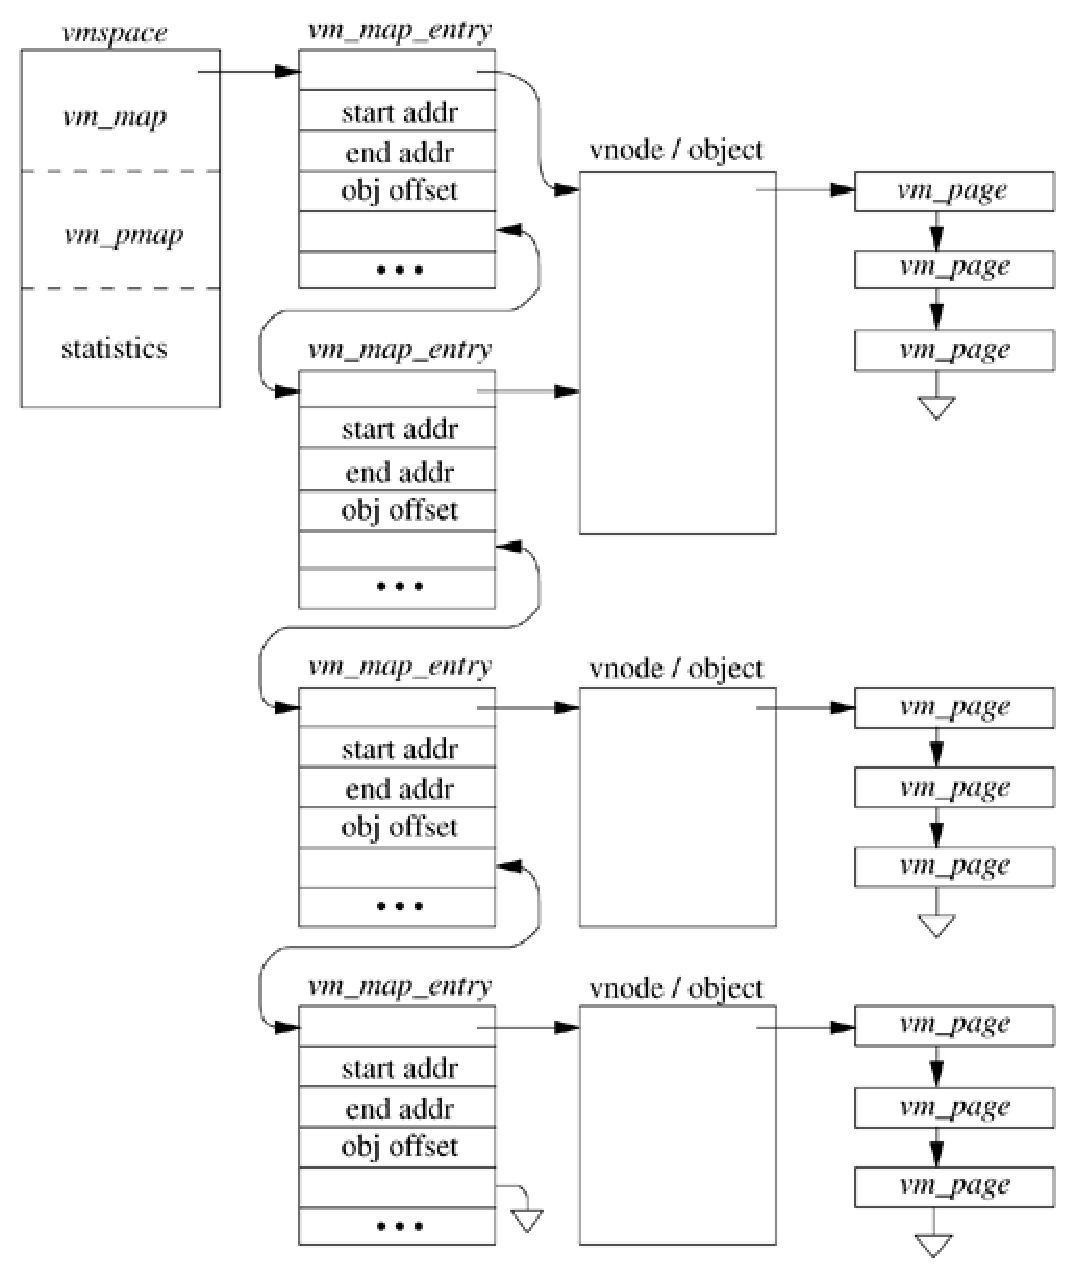
\includegraphics[width=.5\textwidth, height=.35\textheight]{freebsd.eps}
			\centering
			\caption{FreeBSD virtual memory schematic \cite{freeBSDMM}}
			\label{fig:mesh1}
		\end{figure}

		FreeBSD uses the schematic shown in figure 1 to implement virtual memory.
		The \textit{vmspace} structure has a \textit{vm\_map} structure which points to an ordered linked-list of \textit{vm\_map\_entry} nodes.
		Each \textit{vm\_map\_entry} node contains the starting and ending address of the process's contiguous region of virtual memory, as well as the offset from the starting address to the \textit{vm\_object}.
		Each \textit{vm\_object} that a \textit{vm\_map\_entry} points to has the same set of attributes, such as protection level.
		There are zero or more “shadow” \textit{vm\_objects} between a \textit{vm\_map\_entry} and its list of \textit{vm\_object}s.
		A shadow object records changes to the \textit{vm\_object}.
		When a change in memory is made, the shadow object stores a pointer to a new \textit{vm\_page} containing the changes and another pointer to the unmodified \textit{vm\_object}.
		A \textit{vm\_object} node contains a pointer to a linked-list of \textit{vm\_page}s.
		These pages makeup the physical memory cache of the \textit{vm\_object} \cite{freeBSDMM}. 
		
	\subsection{Page Management}
		FreeBSD places pages in one of five states \cite{freeBSDBook}.
		
		\textit{Wired:} Wired pages are locked in memory and can't be paged out.
		A page is in this state when it is in use by the kernel, the physical-memory pager, or a program specifies that the page should be locked via the \textit{mlock} call.
		
		\textit{Active:} Active pages are currently in use by one or more regions of virtual memory.
		
		\textit{Inactive:} Inactive pages are not currently in use and their data is out of date.
		Their data has not been updated to match the new writes in the backing store.
		
		\textit{Cache:} Cache pages contain data that is still in agreement with the backing store but are not currently in use.
		If an active page gets paged-out it will become a cached page.
		Pages in the cached list are similar to those in the \textit{inactive} list, except their contents are known.
		
		\textit{Free:} Free pages are no longer considered useful and will be overwritten.
		
		In summary, \textit{active} and \textit{wired} pages are those which are currently in use and can't be paged out to \textit{free}. 
		\textit{Inactive} pages are out of date and not in use, so they can be paged out.
		\textit{Cache} pages are those that are up to date and not in use.
		\textit{Cache} pages are kept around in case the system needs to page them in again soon.
		\textit{Free} pages are unused and will be overwritten.
		
\section{Windows Implementation}
	\subsection{Memory Manager}	
		Windows has a \textit{memory manager} which handles all tasks related to allocating and managing memory. 
		The memory manager is responsible for fetching the physical memory mapped to by virtual memory, paging contents to disk when they become overcommitted, creating memory mapped files, managing copy-on-write memory, and managing large sparse address spaces \cite{windowsMM}.
		
		At a high level the memory manager handles all of the above in the same manner that Linux does.
		The use of page tables to access a virtual memory's corresponding physical memory is consistent with how Linux performs the translation.
		The \textit{page table} has a \textit{page table index}, \textit{page directory index}, and \textit{byte offset} that the memory manager uses to translate the virtual memory to physical memory.
		
	\subsection{Virtual Memory}
		\begin{figure}[H]
			\includegraphics[width=.6\textwidth, height=.4\textheight]{windowsMM.eps}
			\centering
			\caption{Windows virtual memory schematic \cite{windowsMM}}
			\label{fig:mesh1}
		\end{figure}
		
		Each process has a single \textit{page directory}, created by the memory manager, to map the location of all page tables for that process.
		The page directory is filled with \textit{page directory entries} (PDEs).
		PDEs contain data that describes the state and location of all the possible page tables for the process. 
		
		The memory management unit goes through the workflow below to translate the virtual address to a physical one \cite{windowsMM}.
		\begin{enumerate}
			\item{
				A privileged CPU register, CR3, is used to obtain the physical address of the page directory.
			}
			\item{
				The \textit{page directory index} located in the virtual address (as shown in figure 2) is used as an index into the page directory.}
			\item{
				The \textit{page table index} is used as an index into the page table to locate the PTE.}
			\item{
				If the PTE's \textit{valid bit} is clear, then a page fault occurs and the memory manager attempts to fetch the page.
				If the PTE's \textit{valid bit} is not clear, or the page shouldn't be accessed, then an access violation or bug check is generated}
			\item{
				The physical address is then fetched using the PFN field of the PTE to access the correct page frame.
				Then, the \textit{byte offset} is used to offset into the page frame to the requested physical address.}
	\end{enumerate}
\section{Compare}
	Linux, FreeBSD, and Windows all translate virtual addresses to physical addresses at the granularity of a page.
	This means the smallest unit of protection at the hardware level is a page. 
	I believe this design decision was made because it simplifies virtual-to-physical translation by keeping a uniform memory size.
	
	The three operating systems' virtual-to-physical translation process is roughly the same as well.
	The location of needed indices and the page frame number are stored in different places, but the high level idea is the same.
	I believe all three operating systems use this process because it is efficient (having an index into a table allows for constant lookup) and systematic (easy to follow).
	
	
	
\bibliographystyle{IEEEtran}
\bibliography{references.bib}

\end{document}